\hypertarget{ht__free_8c}{
\section{ht\_\-free.c File Reference}
\label{ht__free_8c}\index{ht_free.c@{ht\_\-free.c}}
}


\subsection{Detailed Description}
\begin{Desc}
\item[For internal use only.]
This file contains the implementation of the \hyperlink{group__dbprim__hash_ga18}{ht\_\-free()} function, used to release memory still in use by an empty hash table.\end{Desc}


Definition in file \hyperlink{ht__free_8c-source}{ht\_\-free.c}.

{\tt \#include $<$stdlib.h$>$}\par
{\tt \#include \char`\"{}dbprim.h\char`\"{}}\par
{\tt \#include \char`\"{}dbprim\_\-int.h\char`\"{}}\par


Include dependency graph for ht\_\-free.c:\begin{figure}[H]
\begin{center}
\leavevmode
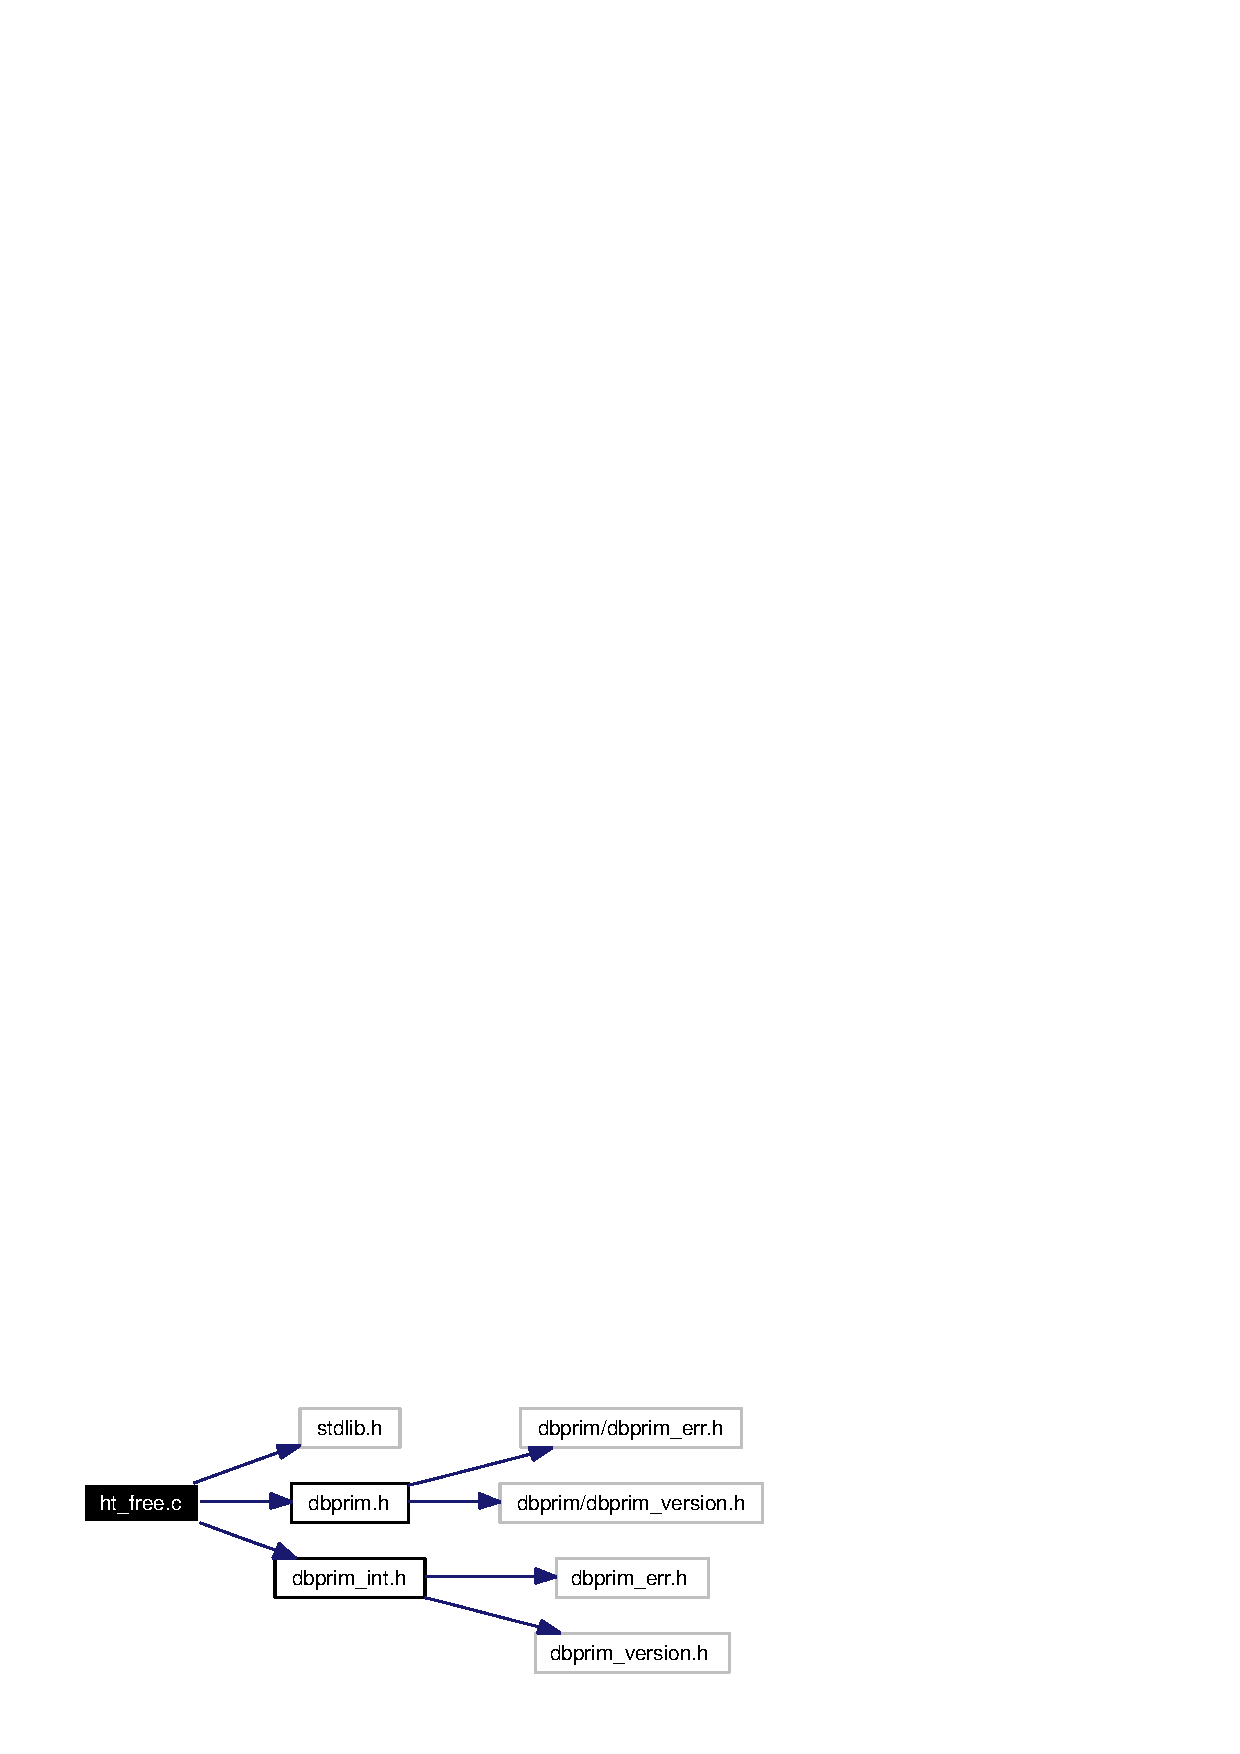
\includegraphics[width=185pt]{ht__free_8c__incl}
\end{center}
\end{figure}
\subsection*{Functions}
\begin{CompactItemize}
\item 
unsigned long \hyperlink{group__dbprim__hash_ga18}{ht\_\-free} (\hyperlink{struct__hash__table__s}{hash\_\-table\_\-t} $\ast$table)
\begin{CompactList}\small\item\em Free memory used by an empty hash table. \item\end{CompactList}\end{CompactItemize}
